% Created by tikzDevice version 0.12.3.1 on 2022-10-04 11:34:14
% !TEX encoding = UTF-8 Unicode
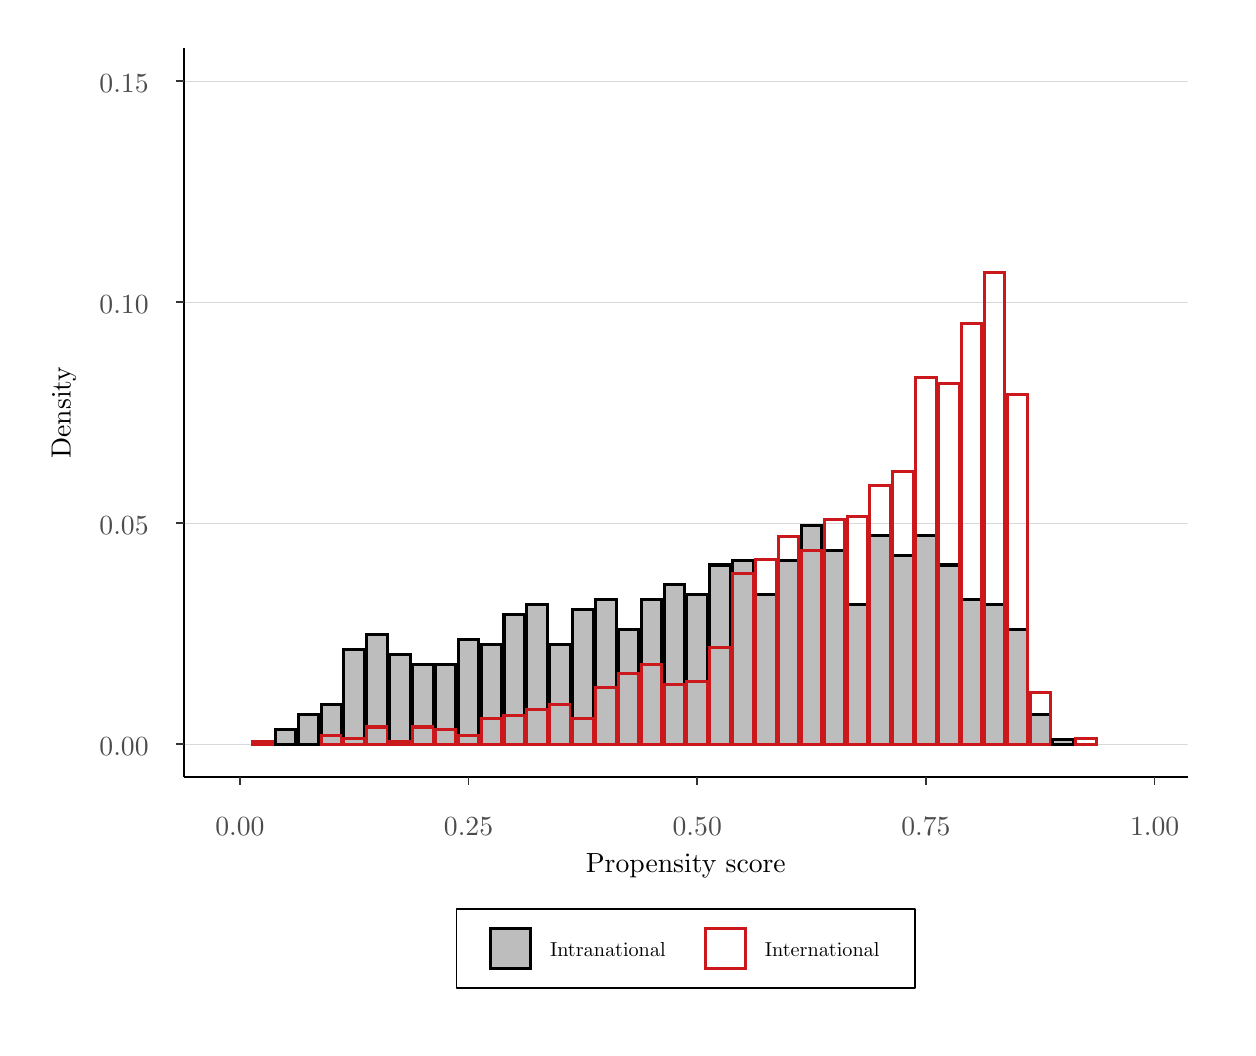
\begin{tikzpicture}[x=1pt,y=1pt]
\definecolor{fillColor}{RGB}{255,255,255}
\path[use as bounding box,fill=fillColor,fill opacity=0.00] (0,0) rectangle (433.62,361.35);
\begin{scope}
\path[clip] (  0.00,  0.00) rectangle (433.62,361.35);
\definecolor{drawColor}{RGB}{255,255,255}
\definecolor{fillColor}{RGB}{255,255,255}

\path[draw=drawColor,line width= 0.6pt,line join=round,line cap=round,fill=fillColor] ( -0.00,  0.00) rectangle (433.62,361.35);
\end{scope}
\begin{scope}
\path[clip] ( 56.47, 90.50) rectangle (419.17,354.12);
\definecolor{drawColor}{RGB}{255,255,255}

\path[draw=drawColor,line width= 0.3pt,line join=round] ( 56.47,142.42) --
	(419.17,142.42);

\path[draw=drawColor,line width= 0.3pt,line join=round] ( 56.47,222.31) --
	(419.17,222.31);

\path[draw=drawColor,line width= 0.3pt,line join=round] ( 56.47,302.20) --
	(419.17,302.20);

\path[draw=drawColor,line width= 0.3pt,line join=round] (117.99, 90.50) --
	(117.99,354.12);

\path[draw=drawColor,line width= 0.3pt,line join=round] (200.63, 90.50) --
	(200.63,354.12);

\path[draw=drawColor,line width= 0.3pt,line join=round] (283.27, 90.50) --
	(283.27,354.12);

\path[draw=drawColor,line width= 0.3pt,line join=round] (365.91, 90.50) --
	(365.91,354.12);
\definecolor{drawColor}{gray}{0.85}

\path[draw=drawColor,line width= 0.1pt,line join=round] ( 56.47,102.48) --
	(419.17,102.48);

\path[draw=drawColor,line width= 0.1pt,line join=round] ( 56.47,182.37) --
	(419.17,182.37);

\path[draw=drawColor,line width= 0.1pt,line join=round] ( 56.47,262.25) --
	(419.17,262.25);

\path[draw=drawColor,line width= 0.1pt,line join=round] ( 56.47,342.14) --
	(419.17,342.14);
\definecolor{drawColor}{RGB}{203,24,29}

\path[draw=drawColor,line width= 1.1pt,line cap=rect] ( 81.22,102.48) rectangle ( 88.65,103.51);
\definecolor{drawColor}{RGB}{0,0,0}
\definecolor{fillColor}{gray}{0.74}

\path[draw=drawColor,line width= 1.1pt,line cap=rect,fill=fillColor] ( 89.48,102.48) rectangle ( 96.92,107.87);

\path[draw=drawColor,line width= 1.1pt,line cap=rect,fill=fillColor] ( 97.74,102.48) rectangle (105.18,113.26);

\path[draw=drawColor,line width= 1.1pt,line cap=rect,fill=fillColor] (106.01,102.48) rectangle (113.44,116.86);
\definecolor{drawColor}{RGB}{203,24,29}

\path[draw=drawColor,line width= 1.1pt,line cap=rect] (106.01,102.48) rectangle (113.44,105.56);
\definecolor{drawColor}{RGB}{0,0,0}

\path[draw=drawColor,line width= 1.1pt,line cap=rect,fill=fillColor] (114.27,102.48) rectangle (121.71,136.63);
\definecolor{drawColor}{RGB}{203,24,29}

\path[draw=drawColor,line width= 1.1pt,line cap=rect] (114.27,102.48) rectangle (121.71,104.53);
\definecolor{drawColor}{RGB}{0,0,0}

\path[draw=drawColor,line width= 1.1pt,line cap=rect,fill=fillColor] (122.54,102.48) rectangle (129.97,142.02);
\definecolor{drawColor}{RGB}{203,24,29}

\path[draw=drawColor,line width= 1.1pt,line cap=rect] (122.54,102.48) rectangle (129.97,108.64);
\definecolor{drawColor}{RGB}{0,0,0}

\path[draw=drawColor,line width= 1.1pt,line cap=rect,fill=fillColor] (130.80,102.48) rectangle (138.24,134.83);
\definecolor{drawColor}{RGB}{203,24,29}

\path[draw=drawColor,line width= 1.1pt,line cap=rect] (130.80,102.48) rectangle (138.24,103.51);
\definecolor{drawColor}{RGB}{0,0,0}

\path[draw=drawColor,line width= 1.1pt,line cap=rect,fill=fillColor] (139.06,102.48) rectangle (146.50,131.24);
\definecolor{drawColor}{RGB}{203,24,29}

\path[draw=drawColor,line width= 1.1pt,line cap=rect] (139.06,102.48) rectangle (146.50,108.64);
\definecolor{drawColor}{RGB}{0,0,0}

\path[draw=drawColor,line width= 1.1pt,line cap=rect,fill=fillColor] (147.33,102.48) rectangle (154.76,131.24);
\definecolor{drawColor}{RGB}{203,24,29}

\path[draw=drawColor,line width= 1.1pt,line cap=rect] (147.33,102.48) rectangle (154.76,107.62);
\definecolor{drawColor}{RGB}{0,0,0}

\path[draw=drawColor,line width= 1.1pt,line cap=rect,fill=fillColor] (155.59,102.48) rectangle (163.03,140.22);
\definecolor{drawColor}{RGB}{203,24,29}

\path[draw=drawColor,line width= 1.1pt,line cap=rect] (155.59,102.48) rectangle (163.03,105.56);
\definecolor{drawColor}{RGB}{0,0,0}

\path[draw=drawColor,line width= 1.1pt,line cap=rect,fill=fillColor] (163.85,102.48) rectangle (171.29,138.43);
\definecolor{drawColor}{RGB}{203,24,29}

\path[draw=drawColor,line width= 1.1pt,line cap=rect] (163.85,102.48) rectangle (171.29,111.72);
\definecolor{drawColor}{RGB}{0,0,0}

\path[draw=drawColor,line width= 1.1pt,line cap=rect,fill=fillColor] (172.12,102.48) rectangle (179.56,149.21);
\definecolor{drawColor}{RGB}{203,24,29}

\path[draw=drawColor,line width= 1.1pt,line cap=rect] (172.12,102.48) rectangle (179.56,112.75);
\definecolor{drawColor}{RGB}{0,0,0}

\path[draw=drawColor,line width= 1.1pt,line cap=rect,fill=fillColor] (180.38,102.48) rectangle (187.82,152.80);
\definecolor{drawColor}{RGB}{203,24,29}

\path[draw=drawColor,line width= 1.1pt,line cap=rect] (180.38,102.48) rectangle (187.82,114.80);
\definecolor{drawColor}{RGB}{0,0,0}

\path[draw=drawColor,line width= 1.1pt,line cap=rect,fill=fillColor] (188.65,102.48) rectangle (196.08,138.43);
\definecolor{drawColor}{RGB}{203,24,29}

\path[draw=drawColor,line width= 1.1pt,line cap=rect] (188.65,102.48) rectangle (196.08,116.86);
\definecolor{drawColor}{RGB}{0,0,0}

\path[draw=drawColor,line width= 1.1pt,line cap=rect,fill=fillColor] (196.91,102.48) rectangle (204.35,151.01);
\definecolor{drawColor}{RGB}{203,24,29}

\path[draw=drawColor,line width= 1.1pt,line cap=rect] (196.91,102.48) rectangle (204.35,111.72);
\definecolor{drawColor}{RGB}{0,0,0}

\path[draw=drawColor,line width= 1.1pt,line cap=rect,fill=fillColor] (205.17,102.48) rectangle (212.61,154.60);
\definecolor{drawColor}{RGB}{203,24,29}

\path[draw=drawColor,line width= 1.1pt,line cap=rect] (205.17,102.48) rectangle (212.61,123.02);
\definecolor{drawColor}{RGB}{0,0,0}

\path[draw=drawColor,line width= 1.1pt,line cap=rect,fill=fillColor] (213.44,102.48) rectangle (220.87,143.82);
\definecolor{drawColor}{RGB}{203,24,29}

\path[draw=drawColor,line width= 1.1pt,line cap=rect] (213.44,102.48) rectangle (220.87,128.15);
\definecolor{drawColor}{RGB}{0,0,0}

\path[draw=drawColor,line width= 1.1pt,line cap=rect,fill=fillColor] (221.70,102.48) rectangle (229.14,154.60);
\definecolor{drawColor}{RGB}{203,24,29}

\path[draw=drawColor,line width= 1.1pt,line cap=rect] (221.70,102.48) rectangle (229.14,131.23);
\definecolor{drawColor}{RGB}{0,0,0}

\path[draw=drawColor,line width= 1.1pt,line cap=rect,fill=fillColor] (229.97,102.48) rectangle (237.40,159.99);
\definecolor{drawColor}{RGB}{203,24,29}

\path[draw=drawColor,line width= 1.1pt,line cap=rect] (229.97,102.48) rectangle (237.40,124.04);
\definecolor{drawColor}{RGB}{0,0,0}

\path[draw=drawColor,line width= 1.1pt,line cap=rect,fill=fillColor] (238.23,102.48) rectangle (245.67,156.40);
\definecolor{drawColor}{RGB}{203,24,29}

\path[draw=drawColor,line width= 1.1pt,line cap=rect] (238.23,102.48) rectangle (245.67,125.07);
\definecolor{drawColor}{RGB}{0,0,0}

\path[draw=drawColor,line width= 1.1pt,line cap=rect,fill=fillColor] (246.49,102.48) rectangle (253.93,167.18);
\definecolor{drawColor}{RGB}{203,24,29}

\path[draw=drawColor,line width= 1.1pt,line cap=rect] (246.49,102.48) rectangle (253.93,137.39);
\definecolor{drawColor}{RGB}{0,0,0}

\path[draw=drawColor,line width= 1.1pt,line cap=rect,fill=fillColor] (254.76,102.48) rectangle (262.19,168.98);
\definecolor{drawColor}{RGB}{203,24,29}

\path[draw=drawColor,line width= 1.1pt,line cap=rect] (254.76,102.48) rectangle (262.19,164.09);
\definecolor{drawColor}{RGB}{0,0,0}

\path[draw=drawColor,line width= 1.1pt,line cap=rect,fill=fillColor] (263.02,102.48) rectangle (270.46,156.40);
\definecolor{drawColor}{RGB}{203,24,29}

\path[draw=drawColor,line width= 1.1pt,line cap=rect] (263.02,102.48) rectangle (270.46,169.22);
\definecolor{drawColor}{RGB}{0,0,0}

\path[draw=drawColor,line width= 1.1pt,line cap=rect,fill=fillColor] (271.28,102.48) rectangle (278.72,168.98);
\definecolor{drawColor}{RGB}{203,24,29}

\path[draw=drawColor,line width= 1.1pt,line cap=rect] (271.28,102.48) rectangle (278.72,177.44);
\definecolor{drawColor}{RGB}{0,0,0}

\path[draw=drawColor,line width= 1.1pt,line cap=rect,fill=fillColor] (279.55,102.48) rectangle (286.99,181.56);
\definecolor{drawColor}{RGB}{203,24,29}

\path[draw=drawColor,line width= 1.1pt,line cap=rect] (279.55,102.48) rectangle (286.99,172.30);
\definecolor{drawColor}{RGB}{0,0,0}

\path[draw=drawColor,line width= 1.1pt,line cap=rect,fill=fillColor] (287.81,102.48) rectangle (295.25,172.57);
\definecolor{drawColor}{RGB}{203,24,29}

\path[draw=drawColor,line width= 1.1pt,line cap=rect] (287.81,102.48) rectangle (295.25,183.60);
\definecolor{drawColor}{RGB}{0,0,0}

\path[draw=drawColor,line width= 1.1pt,line cap=rect,fill=fillColor] (296.08,102.48) rectangle (303.51,152.80);
\definecolor{drawColor}{RGB}{203,24,29}

\path[draw=drawColor,line width= 1.1pt,line cap=rect] (296.08,102.48) rectangle (303.51,184.63);
\definecolor{drawColor}{RGB}{0,0,0}

\path[draw=drawColor,line width= 1.1pt,line cap=rect,fill=fillColor] (304.34,102.48) rectangle (311.78,177.96);
\definecolor{drawColor}{RGB}{203,24,29}

\path[draw=drawColor,line width= 1.1pt,line cap=rect] (304.34,102.48) rectangle (311.78,195.92);
\definecolor{drawColor}{RGB}{0,0,0}

\path[draw=drawColor,line width= 1.1pt,line cap=rect,fill=fillColor] (312.60,102.48) rectangle (320.04,170.78);
\definecolor{drawColor}{RGB}{203,24,29}

\path[draw=drawColor,line width= 1.1pt,line cap=rect] (312.60,102.48) rectangle (320.04,201.06);
\definecolor{drawColor}{RGB}{0,0,0}

\path[draw=drawColor,line width= 1.1pt,line cap=rect,fill=fillColor] (320.87,102.48) rectangle (328.30,177.96);
\definecolor{drawColor}{RGB}{203,24,29}

\path[draw=drawColor,line width= 1.1pt,line cap=rect] (320.87,102.48) rectangle (328.30,234.94);
\definecolor{drawColor}{RGB}{0,0,0}

\path[draw=drawColor,line width= 1.1pt,line cap=rect,fill=fillColor] (329.13,102.48) rectangle (336.57,167.18);
\definecolor{drawColor}{RGB}{203,24,29}

\path[draw=drawColor,line width= 1.1pt,line cap=rect] (329.13,102.48) rectangle (336.57,232.89);
\definecolor{drawColor}{RGB}{0,0,0}

\path[draw=drawColor,line width= 1.1pt,line cap=rect,fill=fillColor] (337.40,102.48) rectangle (344.83,154.60);
\definecolor{drawColor}{RGB}{203,24,29}

\path[draw=drawColor,line width= 1.1pt,line cap=rect] (337.40,102.48) rectangle (344.83,254.45);
\definecolor{drawColor}{RGB}{0,0,0}

\path[draw=drawColor,line width= 1.1pt,line cap=rect,fill=fillColor] (345.66,102.48) rectangle (353.10,152.80);
\definecolor{drawColor}{RGB}{203,24,29}

\path[draw=drawColor,line width= 1.1pt,line cap=rect] (345.66,102.48) rectangle (353.10,272.93);
\definecolor{drawColor}{RGB}{0,0,0}

\path[draw=drawColor,line width= 1.1pt,line cap=rect,fill=fillColor] (353.92,102.48) rectangle (361.36,143.82);
\definecolor{drawColor}{RGB}{203,24,29}

\path[draw=drawColor,line width= 1.1pt,line cap=rect] (353.92,102.48) rectangle (361.36,228.78);
\definecolor{drawColor}{RGB}{0,0,0}

\path[draw=drawColor,line width= 1.1pt,line cap=rect,fill=fillColor] (362.19,102.48) rectangle (369.62,113.26);
\definecolor{drawColor}{RGB}{203,24,29}

\path[draw=drawColor,line width= 1.1pt,line cap=rect] (362.19,102.48) rectangle (369.62,120.96);
\definecolor{drawColor}{RGB}{0,0,0}

\path[draw=drawColor,line width= 1.1pt,line cap=rect,fill=fillColor] (370.45,102.48) rectangle (377.89,104.28);
\definecolor{drawColor}{RGB}{203,24,29}

\path[draw=drawColor,line width= 1.1pt,line cap=rect] (378.71,102.48) rectangle (386.15,104.53);
\end{scope}
\begin{scope}
\path[clip] (  0.00,  0.00) rectangle (433.62,361.35);
\definecolor{drawColor}{RGB}{0,0,0}

\path[draw=drawColor,line width= 0.6pt,line join=round] ( 56.47, 90.50) --
	( 56.47,354.12);
\end{scope}
\begin{scope}
\path[clip] (  0.00,  0.00) rectangle (433.62,361.35);
\definecolor{drawColor}{gray}{0.30}

\node[text=drawColor,anchor=base east,inner sep=0pt, outer sep=0pt, scale=  1.00] at ( 43.72, 98.35) {0.00};

\node[text=drawColor,anchor=base east,inner sep=0pt, outer sep=0pt, scale=  1.00] at ( 43.72,178.23) {0.05};

\node[text=drawColor,anchor=base east,inner sep=0pt, outer sep=0pt, scale=  1.00] at ( 43.72,258.12) {0.10};

\node[text=drawColor,anchor=base east,inner sep=0pt, outer sep=0pt, scale=  1.00] at ( 43.72,338.01) {0.15};
\end{scope}
\begin{scope}
\path[clip] (  0.00,  0.00) rectangle (433.62,361.35);
\definecolor{drawColor}{gray}{0.20}

\path[draw=drawColor,line width= 0.6pt,line join=round] ( 53.72,102.48) --
	( 56.47,102.48);

\path[draw=drawColor,line width= 0.6pt,line join=round] ( 53.72,182.37) --
	( 56.47,182.37);

\path[draw=drawColor,line width= 0.6pt,line join=round] ( 53.72,262.25) --
	( 56.47,262.25);

\path[draw=drawColor,line width= 0.6pt,line join=round] ( 53.72,342.14) --
	( 56.47,342.14);
\end{scope}
\begin{scope}
\path[clip] (  0.00,  0.00) rectangle (433.62,361.35);
\definecolor{drawColor}{RGB}{0,0,0}

\path[draw=drawColor,line width= 0.6pt,line join=round] ( 56.47, 90.50) --
	(419.17, 90.50);
\end{scope}
\begin{scope}
\path[clip] (  0.00,  0.00) rectangle (433.62,361.35);
\definecolor{drawColor}{gray}{0.20}

\path[draw=drawColor,line width= 0.6pt,line join=round] ( 76.67, 87.75) --
	( 76.67, 90.50);

\path[draw=drawColor,line width= 0.6pt,line join=round] (159.31, 87.75) --
	(159.31, 90.50);

\path[draw=drawColor,line width= 0.6pt,line join=round] (241.95, 87.75) --
	(241.95, 90.50);

\path[draw=drawColor,line width= 0.6pt,line join=round] (324.59, 87.75) --
	(324.59, 90.50);

\path[draw=drawColor,line width= 0.6pt,line join=round] (407.22, 87.75) --
	(407.22, 90.50);
\end{scope}
\begin{scope}
\path[clip] (  0.00,  0.00) rectangle (433.62,361.35);
\definecolor{drawColor}{gray}{0.30}

\node[text=drawColor,anchor=base,inner sep=0pt, outer sep=0pt, scale=  1.00] at ( 76.67, 69.48) {0.00};

\node[text=drawColor,anchor=base,inner sep=0pt, outer sep=0pt, scale=  1.00] at (159.31, 69.48) {0.25};

\node[text=drawColor,anchor=base,inner sep=0pt, outer sep=0pt, scale=  1.00] at (241.95, 69.48) {0.50};

\node[text=drawColor,anchor=base,inner sep=0pt, outer sep=0pt, scale=  1.00] at (324.59, 69.48) {0.75};

\node[text=drawColor,anchor=base,inner sep=0pt, outer sep=0pt, scale=  1.00] at (407.22, 69.48) {1.00};
\end{scope}
\begin{scope}
\path[clip] (  0.00,  0.00) rectangle (433.62,361.35);
\definecolor{drawColor}{RGB}{0,0,0}

\node[text=drawColor,anchor=base,inner sep=0pt, outer sep=0pt, scale=  1.00] at (237.82, 56.13) {Propensity score};
\end{scope}
\begin{scope}
\path[clip] (  0.00,  0.00) rectangle (433.62,361.35);
\definecolor{drawColor}{RGB}{0,0,0}

\node[text=drawColor,rotate= 90.00,anchor=base,inner sep=0pt, outer sep=0pt, scale=  1.00] at ( 15.49,222.31) {Density};
\end{scope}
\begin{scope}
\path[clip] (  0.00,  0.00) rectangle (433.62,361.35);
\definecolor{drawColor}{RGB}{0,0,0}
\definecolor{fillColor}{RGB}{255,255,255}

\path[draw=drawColor,line width= 0.6pt,line join=round,line cap=round,fill=fillColor] (154.91, 14.45) rectangle (320.72, 42.80);
\end{scope}
\begin{scope}
\path[clip] (  0.00,  0.00) rectangle (433.62,361.35);

\path[] (165.91, 19.95) rectangle (183.25, 37.30);
\end{scope}
\begin{scope}
\path[clip] (  0.00,  0.00) rectangle (433.62,361.35);
\definecolor{drawColor}{RGB}{0,0,0}
\definecolor{fillColor}{gray}{0.74}

\path[draw=drawColor,line width= 1.1pt,line cap=rect,fill=fillColor] (167.33, 21.38) rectangle (181.83, 35.88);
\end{scope}
\begin{scope}
\path[clip] (  0.00,  0.00) rectangle (433.62,361.35);

\path[] (243.56, 19.95) rectangle (260.90, 37.30);
\end{scope}
\begin{scope}
\path[clip] (  0.00,  0.00) rectangle (433.62,361.35);
\definecolor{drawColor}{RGB}{203,24,29}

\path[draw=drawColor,line width= 1.1pt,line cap=rect] (244.98, 21.38) rectangle (259.48, 35.88);
\end{scope}
\begin{scope}
\path[clip] (  0.00,  0.00) rectangle (433.62,361.35);
\definecolor{drawColor}{RGB}{0,0,0}

\node[text=drawColor,anchor=base west,inner sep=0pt, outer sep=0pt, scale=  0.73] at (188.75, 25.60) {Intranational};
\end{scope}
\begin{scope}
\path[clip] (  0.00,  0.00) rectangle (433.62,361.35);
\definecolor{drawColor}{RGB}{0,0,0}

\node[text=drawColor,anchor=base west,inner sep=0pt, outer sep=0pt, scale=  0.73] at (266.40, 25.60) {International};
\end{scope}
\end{tikzpicture}
